\section{Definition}
\textbf{MapReduce} is a \textbf{popular programming model} designed to \textbf{easily process and generate large datasets on clusters of commodity machines}. Through this paradigm, a computation can be expressed in terms of a \textbf{map and reduce functions} while \textbf{the underlying system deals with communication, parallelization and error handling}, making it easy to use even for programmers who have no experience with distributed systems.

\textbf{Google} created this paradigm in \textbf{2003} in order to reduce development time and cost on their projects; after an analysis of the problem, Google's engineers noticed how \textbf{the majority of the computations in their products could be expressed through the map and reduce abstractions} that are typically present in \textbf{functional languages}. The MapReduce paradigm has been \textbf{used in a variety of Google's project}, including the indexing system used by the Google search engine \cite{google_mapreduce}.

\textbf{\href{https://hadoop.apache.org/}{Apache Hadoop}}, inspired by Google's work, integrates the MapReduce paradigm in its free-licensed framework, making it \textbf{one of the most used options} when it comes to applying distributed computations following this paradigm.

\subsection{The programming model}
TODO
% including types

\subsection{Execution flow}
TODO

\begin{figure}[H]
    \centering
    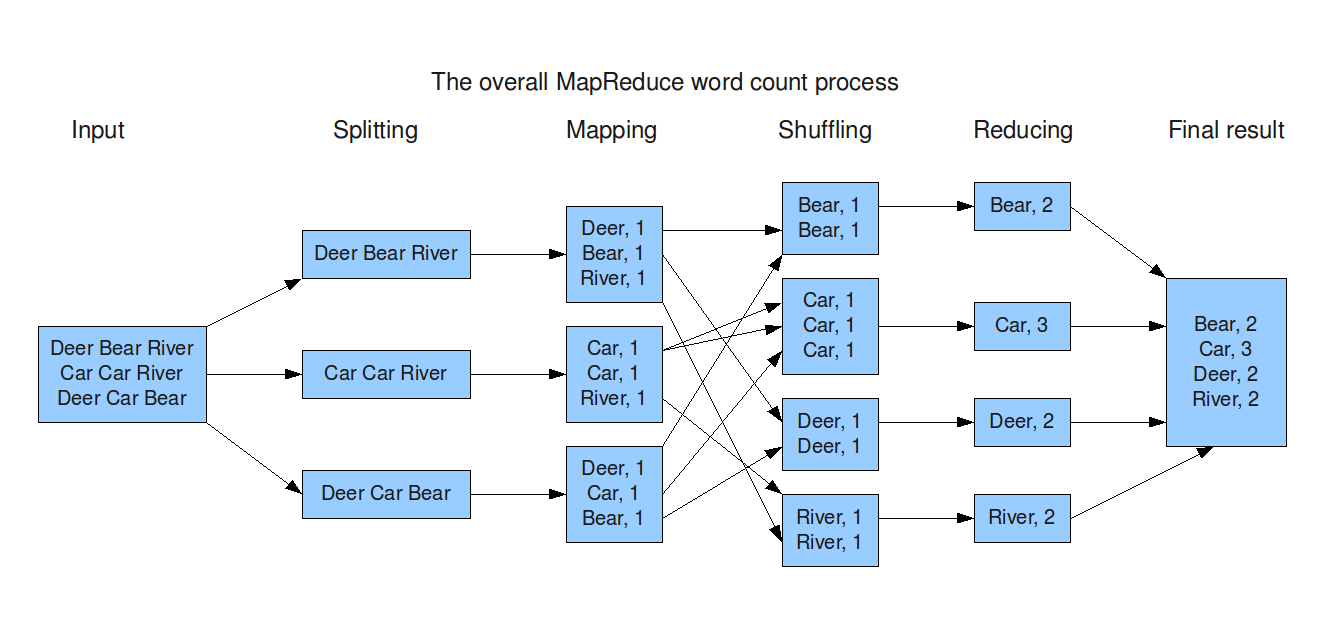
\includegraphics[width=\linewidth]{document/chapters/chapter_4/images/mapreduce_example.png}
    \caption{Example of word count expressed through the MapReduce paradigm \cite{mapreduce_example_site}}
    \label{fig:mapreduce_example}
\end{figure}

\begin{figure}[H]
    \centering
    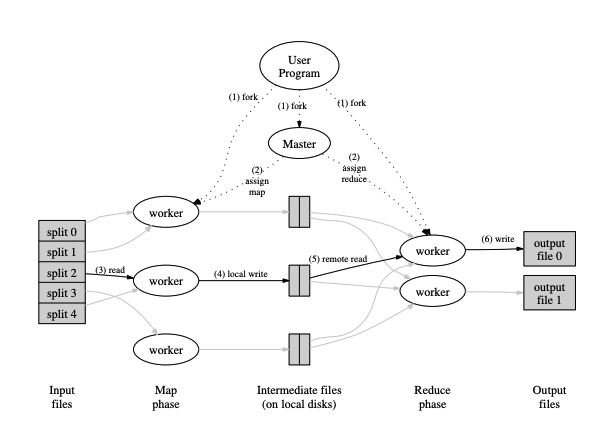
\includegraphics[width=\linewidth]{document/chapters/chapter_4/images/mapreduce_execution_flow.png}
    \caption{MapReduce execution flow \cite{google_mapreduce}}
    \label{fig:mapreduce_execution_flow}
\end{figure}

\subsection{Underlying mechanisms}
TODO

\subsubsection{Data structures}
TODO

\subsubsection{Task granularity}
TODO
% including locality

\subsubsection{Fault tolerance}
TODO
